\chapter{Discussion} \label{sec:discussion}


\section{Conclusion}
From the results presented in \autoref{sec:results}, we can conclude the following.

Firstly, the method is able to model the transformer core in a way that is consistent with the physical properties of the core material. This is shown by the fact that the magnetic flux density in the core is inversely proportional to the permeability of the core material. Consequently, the model correctly captures the behaviour of the core at loads close to the saturation point, as seen by the fact that the magnetic flux density in the core is constant across the cross section of the core. This directly shows that the linear model is not able to capture the behaviour of the core at loads close to the saturation point.

Furthermore, this model does not make any assumptions on the underlying frequency of the magnetic vector potential. As a result, the model can also be easily adapted to model higher and multiple frequencies, as well as multiple frequencies, correctly. As the non-linearities disallow separation of variables in the frequency domain, this is an improvement over the previous work. \todo{Rewrite}

\section{Future work}
The model presented in this paper is a first step towards a more accurate model of the magnetic field in a distribution transformer. However, there are still some improvements that can be made.
\vspace{5pt}

% Frequencies
\noindent This paper only presents results for a single frequency. In theory, the model is also valid for higher, as well as multiple frequencies. However, the model is not yet validated for these cases. Therefore, more research is needed to determine the validity of the model for these cases.

% Optimization
\vspace{5pt}
\noindent At this moment, the model is not fully optimized. As a result, the execution time is quite long. If this is to be used to model a longer time horizon, the execution time needs to be reduced. Some steps in this direction have already been taken:
\begin{itemize}
    \item Matrices have been implemented in a sparse format, which reduces the memory usage and the number of operations needed to perform the matrix-vector multiplications.
    \item A data structure \verb|FastSparse| has been implemented, that efficiently allocates memory for initializing the (sparse) matrices $M$ and $K$.
    \item The assembly of the matrices $M$ and $K$ has been optimized to use to least amount of memory allocations possible.
\end{itemize}
However, there are still some steps that can be taken to further reduce the execution time:
\begin{itemize}
    \item Efficient linear system solver: the current linear system solver is not very efficient. This could be an iterative method, or a Krylov subspace method.
    \item Backward Euler is used to time-step. This could be done more accurately by using a higher order method, such as the Runge-Kutta method, further improving execution time.
\end{itemize}


% Parameter analysis
\vspace{5pt}
\noindent Furthermore, the parameters used in the model are not in agreement with reality. For instance, the core does not operate close to saturation in reality, but at much lower flux densities. Most parameters are estimated based on \cite{vanDijk2022}, and might therefore not be accurate. More research is needed to determine the correct parameters.

% Hybrid mesh
\vspace{5pt}
\noindent Finally, the mesh used in this paper can be improved. The mesh used in this paper is a triangular mesh, and lacks detail to correctly address the skin effect that arises at higher frequencies. \Cref{tab:skin_effect} shows the skin effect for different frequencies. As can be seen, the skin effect is not present at $50$ Hz, but its contribution increases with frequency. Therefore, a hybrid mesh can be used, where the mesh is refined near the edges of the transformer, where the skin effect is most prominent. This will increase the accuracy of the model at higher frequencies. This mesh is shown in \cref{fig:mesh_hybrid}.

\begin{figure}
    \centering
    \begin{multicols}{2}
        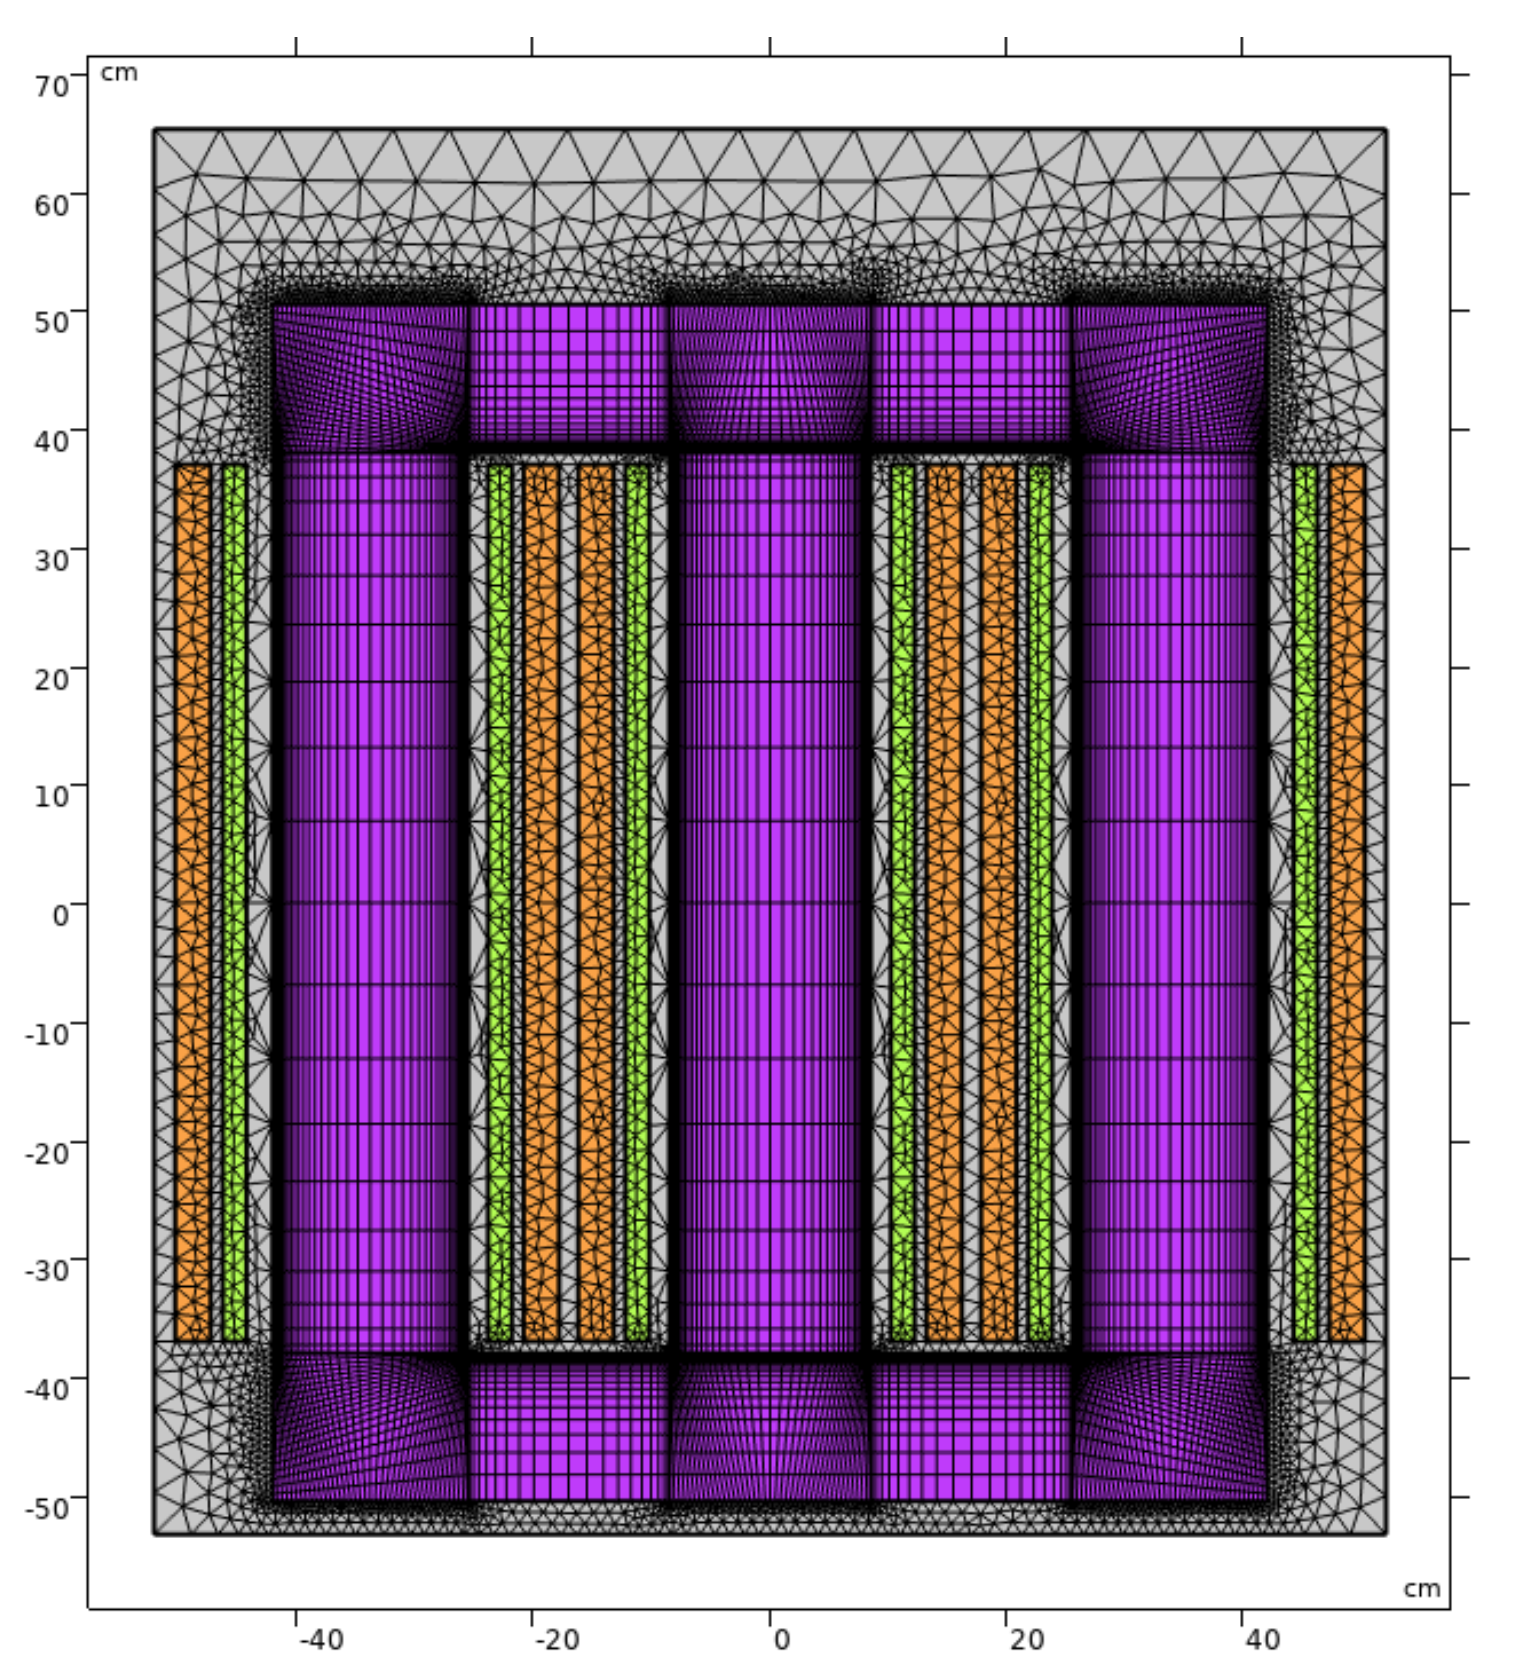
\includegraphics[width=0.45\textwidth]{img/hybrid_mesh_full.png}
        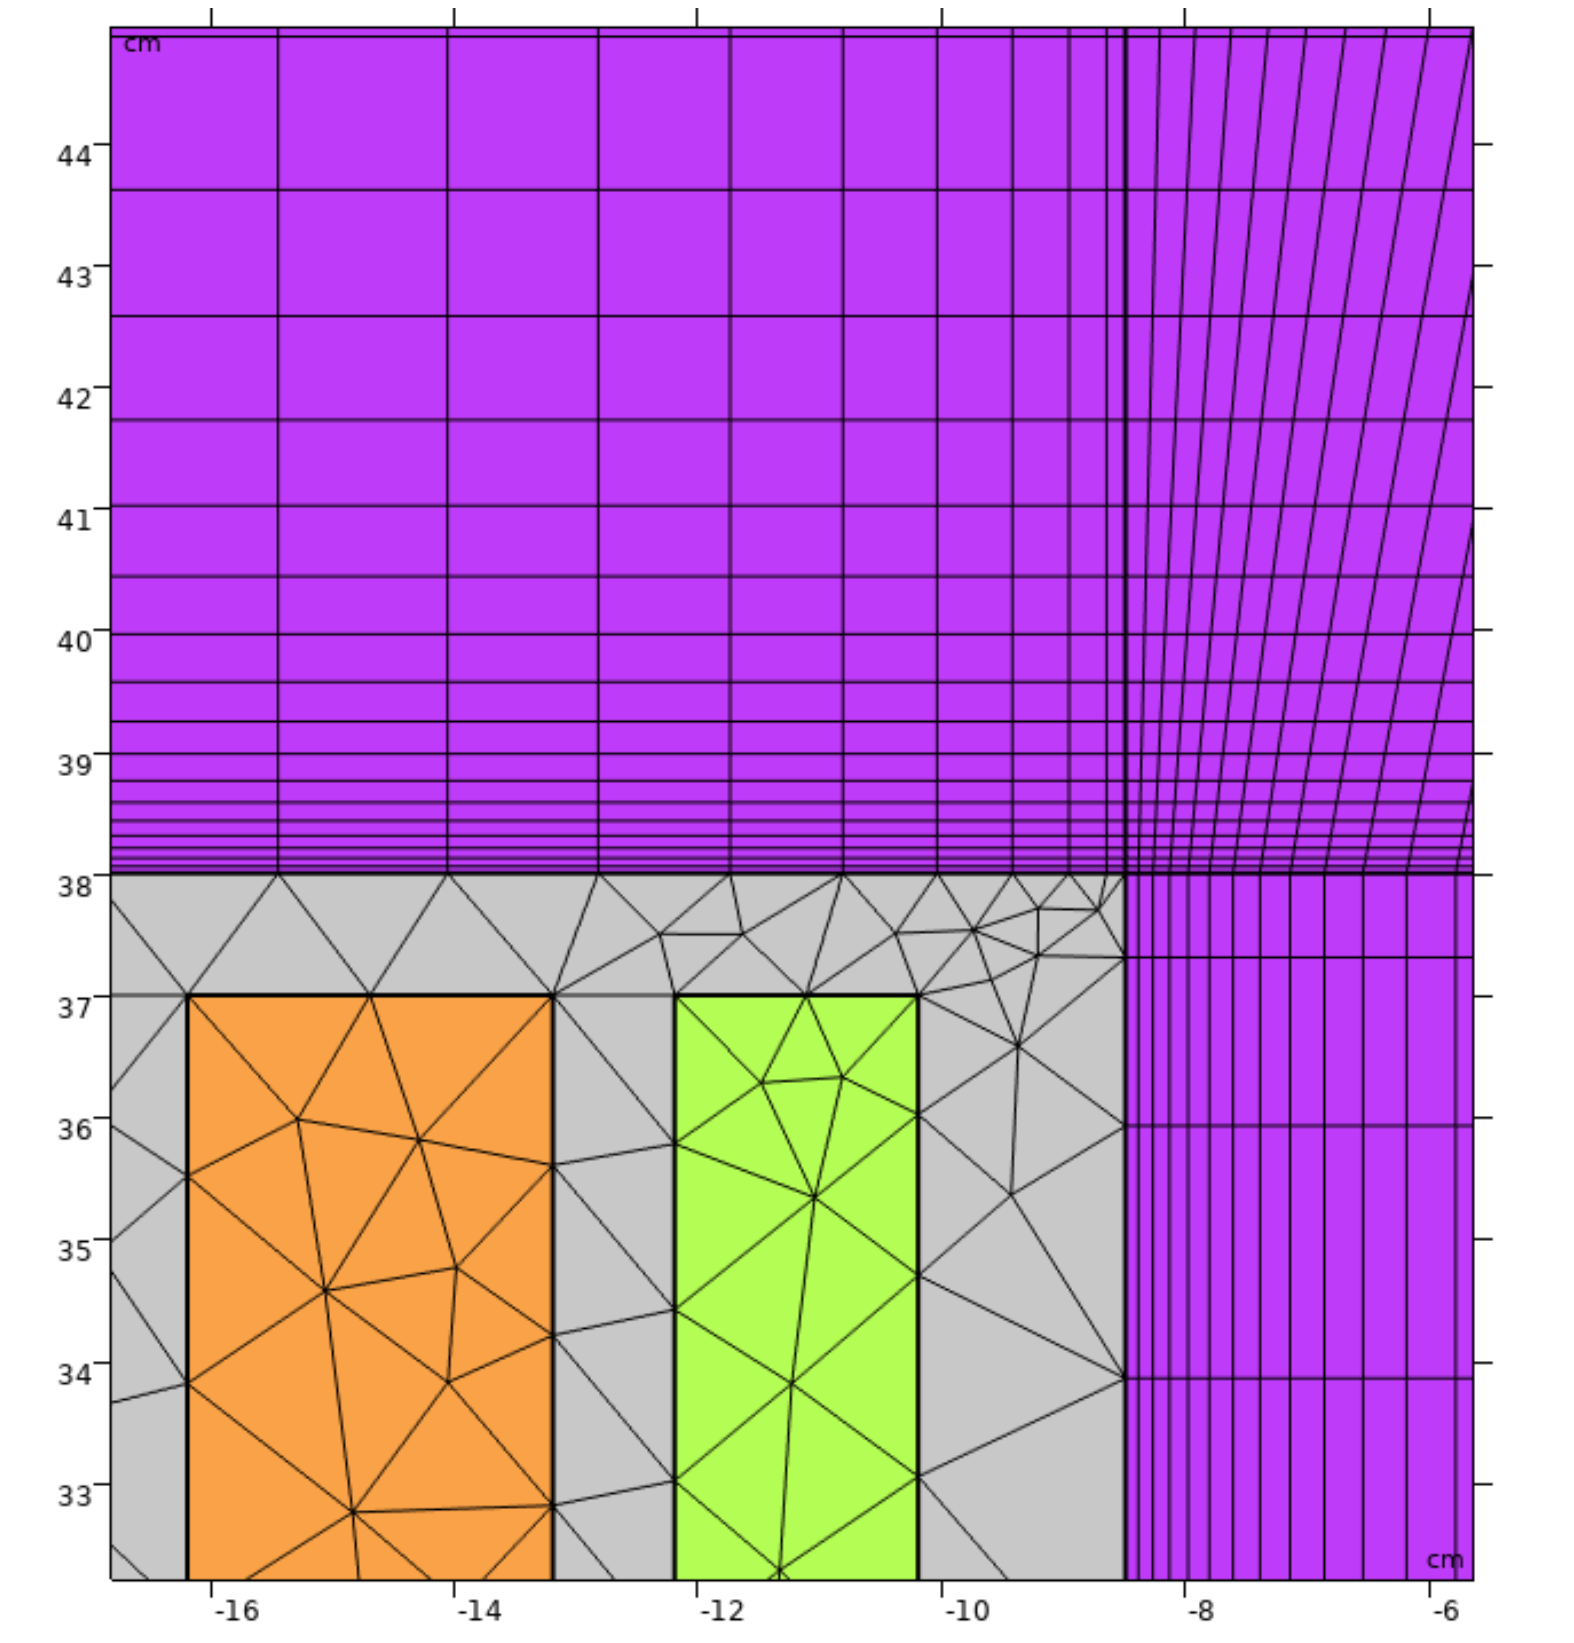
\includegraphics[width=0.45\textwidth]{img/hybrid_mesh.png}
    \end{multicols}
    \caption{Hybrid mesh that can be used to accurately model the skin effect (\cite{vanDijk2022}).}
    \label{fig:mesh_hybrid}
\end{figure}